\subsection{Проектирование и реализация моделей базы данных}
\label{sub:system-design:database-model}

Реляционные системы управления базами данных являются стандартным подходом при проектировании веб-приложений, поскольку удовлетворяют следующим критериям:

\begin{itemize}
    \item поддержание полноты и целостности хранимых данных за счет механизмов уникальности данных, внешних и первичных ключей, наложения ограничений на данные и контроля их связности;
    \item поддержка свойства транзакционности, позволяющее выполнять нес\-коль\-ко операций как неделимое действие и возвращать данные в прошлое состояние в случае провала фиксации данных;
    \item поддержка требований \textit{ACID}: \textit{Atomicity} (атомарность), \textit{Consistency} (согласованность), \textit{Isolation} (изоляция) и \textit{Durability} (долговечность), которые обеспечивают надежность обработки данных.
\end{itemize}

В реализуемой системе структура базы данных представляет собой комплексное решение для управления офисными помещениями, информацией о сотрудниках, контролем доступа и посещаемости, и распределением рабочих мест. 

Как было упомянуто в разделе~\ref{sub:system-design:architectural-pattern-design} на странице~\pageref{page:system-design:architectural-pattern-design:microservices-list}, используемый подход микросервисной архитектуры предполагает наличие нескольких приватных баз данных для каждого сервиса, что обеспечивает изоляцию данных и независимость компонентов. Такой подход позволяет каждому сервису самостоятельно управлять своей схемой данных и выбирать наиболее подходящую технологию хранения, соответствующую специфике бизнес-логики. Разделение данных способствует более четкому разграничению ответственности между командами разработки, а также усиливает инкапсуляцию, предотвращая нежелательные зависимости на уровне базы данных. Кроме того, отказ от общей базы данных позволяет избежать узких мест, связанных с централизованным управлением транзакциями, и минимизировать влияние изменений схемы данных одного сервиса на другие. Такой подход был выбран для обеспечения гибкости системы в условиях высокой нагрузки, а также для упрощения сопровождения и эволюции сервисов в рамках распределенной архитектуры.

Логическая модель базы данных представляется в виде \textit{ER}-модели данных, которая предназначена для описания объектов и отношений базы данных. Основными понятиями модели \textit{ER} являются: сущность (\textit{entity})~-- объект, который идентифицируется человеком конкретно в предметной области; атрибуты~-- значимые характеристики сущности; связи~-- отношения между различными сущностями. На рис.~\ref{fig:system-design:database-model:erd} представлена схема базы данных.

\afterpage{
    \clearpage
    \begin{landscape}
        \thispagestyle{landscape}
        \begin{figure}[p]
            \centering
            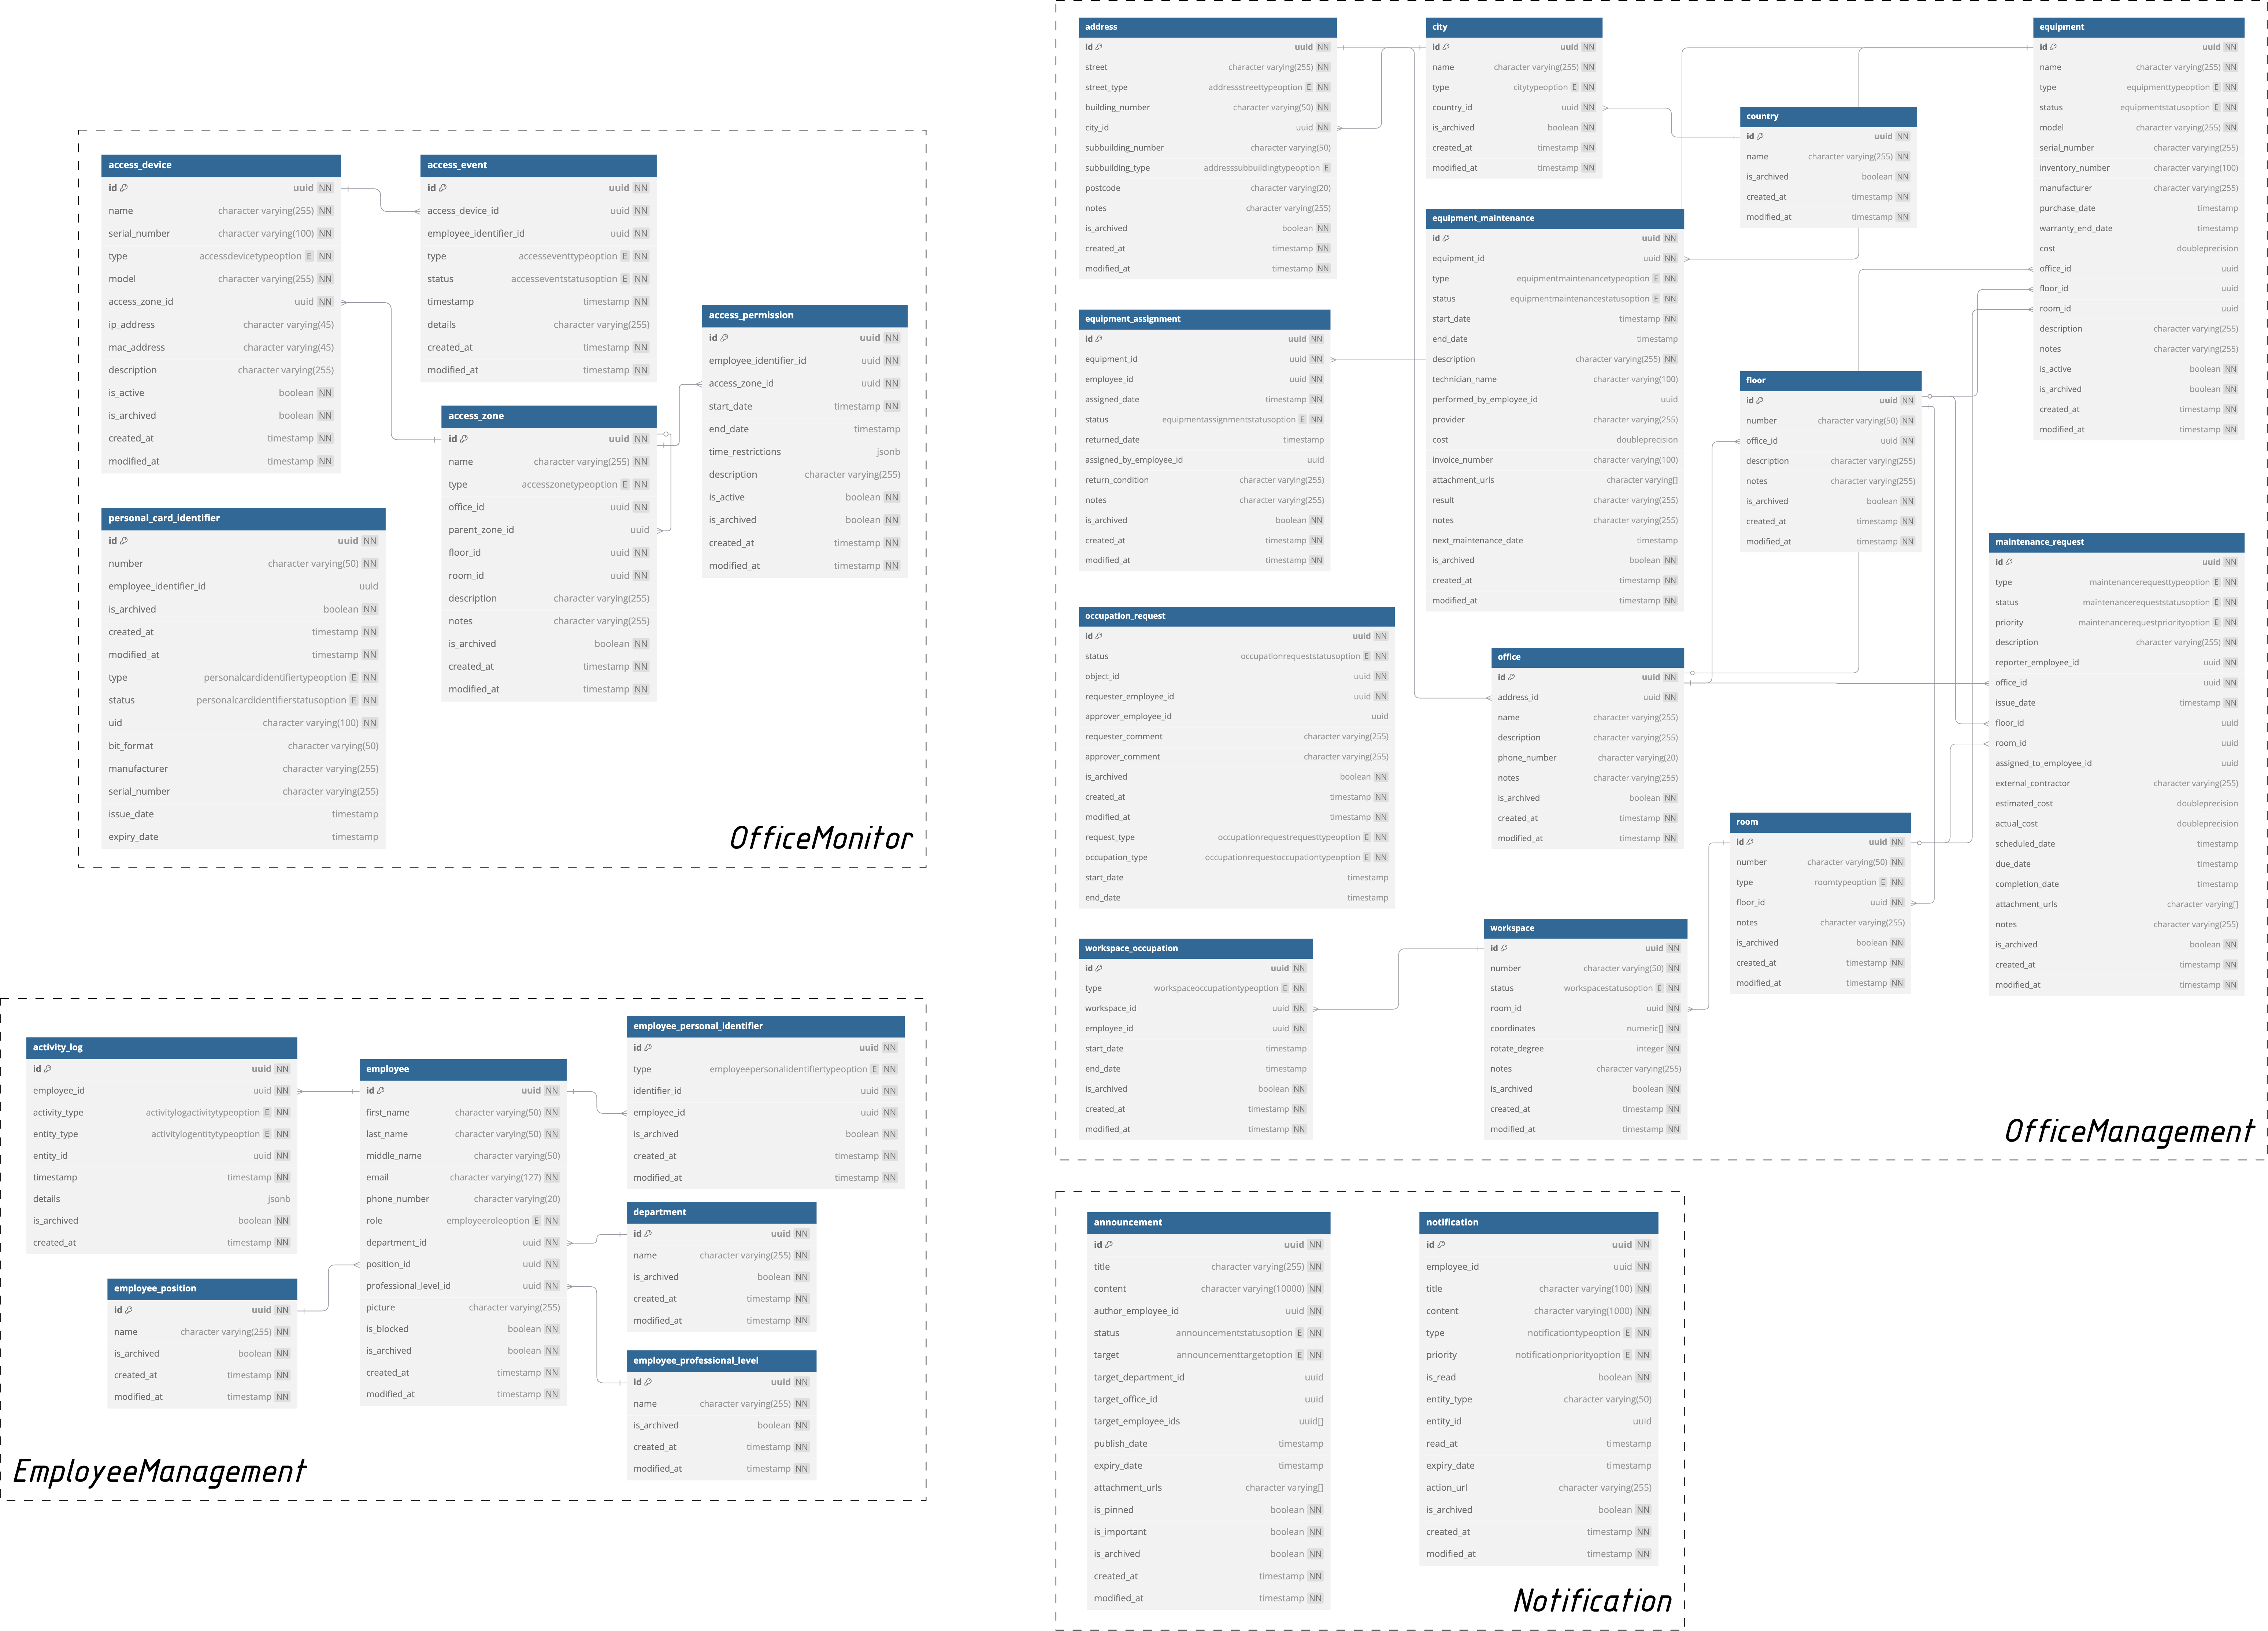
\includegraphics[width=0.8\linewidth]{assets/ERD.png}
            \caption{Схема базы данных}
            \label{fig:system-design:database-model:erd}
        \end{figure}
    \end{landscape}
    \clearpage
}

Рассмотрим структуру базы данных сервиса \textbf{\textit{EmployeeManagement}}, реализующего бизнес-логику операций управления сотрудниками, авторизации и аутентификации в системе. Записи о сотрудниках включают контактную информацию, положение в организации, набор прав и привилегий, и профессиональные атрибуты.

Организационная структура: Отдел → Сотрудник → Должность/профессиональный уровень. Система управления сотрудниками фиксирует отношения подчинения, пути профессионального развития и организацию отдела. Это позволяет выполнять такие \textit{HR}-функции, как составление организационных схем и отслеживание карьерного роста. В таблицах~\ref{table:system-design:database-model:employee-schema},~\ref{table:system-design:database-model:activity_log-schema} представлено подробное описание типов для таблиц «Сотрудник», «Действие» базы данных сервиса \textit{EmployeeManagement}.

Сотрудник занимает определённую должность и имеет установленный профессиональный уровень, а также принадлежит к отделу. Каждому сотруднику соответствует уникальная запись с контактной информацией и ролью в компании. Все действия сотрудников фиксируются в журнале активности, где указывается тип действия, над какой сущностью оно выполнено и дополнительные детали. В таблице «Действие» хранится ссылка на сотрудника, совершившего действие, через внешний ключ. Таким образом, можно отследить, какие действия выполнял конкретный сотрудник. Связи между таблицами обеспечиваются внешними ключами с ограничением на удаление \textit{RESTRICT}, что предотвращает потерю важной информации. Эти взаимосвязи позволяют контролировать активность персонала, а также структурировать и анализировать поведение сотрудников по должности, отделу и уровню.

\begingroup
\singlespacing
\vspace{-\baselineskip}
\begin{longtable}{| >{\raggedright}m{0.29\textwidth} 
                  | >{\raggedright}m{0.35\textwidth} 
                  | >{\raggedright}m{0.15\textwidth} 
                  | >{\raggedright\arraybackslash}m{0.1\textwidth}|}
    \caption{Типы данных сущности «Сотрудник»} \label{table:system-design:database-model:employee-schema} \\ \hline
    Атрибут & Название & Тип & Размер \\ \hline
    \endfirsthead
    \multicolumn{4}{@{}l}{\noindent Продолжение таблицы~\thetable} \\ \hline
    Атрибут & Название & Тип & Размер \\ \hline
    \endhead
    \textit{id} & Идентификатор & \textit{UUID} & - \\ \hline
    \textit{first\_name} & Имя & Строка & 50 \\ \hline
    \textit{last\_name} & Фамилия & Строка & 50 \\ \hline
    \textit{middle\_name} & Отчество & Строка & 50 \\ \hline
    \textit{email} & Адрес электронной почты & Строка & 127 \\ \hline
    \textit{phone\_number} & Номер телефона & Строка & 20 \\ \hline
    \textit{role} & Роль сотрудника & Строка & 15 \\ \hline
    \textit{department\_id} & Внешний ключ на столбец \textit{ID} в таблице «Отдел» & \textit{UUID} & - \\ \hline
    \textit{position\_id} & Внешний ключ на столбец \textit{ID} в таблице «Должность» & \textit{UUID} & - \\ \hline
    \textit{professional\_level\_id} & Внешний ключ на столбец \textit{ID} в таблице «Профессиональный уровень» & \textit{UUID} & - \\ \hline
    \textit{picture} & Путь к изображению (ссылка) & Строка & 255 \\ \hline
    \textit{is\_blocked} & Флаг блокировки сотрудника & Булево & - \\ \hline
    \textit{is\_archived} & Флаг архивирования записи сотрудника & Булево & - \\ \hline
    \textit{created\_at} & Временная метка создания записи & Дата и время & - \\ \hline
    \textit{modified\_at} & Временная метка изменения записи & Дата и время & - \\ \hline
\end{longtable}
\endgroup

\begingroup
\singlespacing
\vspace{-\baselineskip}
\begin{longtable}{| >{\raggedright}m{0.29\textwidth} 
                  | >{\raggedright}m{0.35\textwidth} 
                  | >{\raggedright}m{0.15\textwidth} 
                  | >{\raggedright\arraybackslash}m{0.1\textwidth}|}
    \caption{Типы данных сущности «Действие»} \label{table:system-design:database-model:activity_log-schema} \\ \hline
    Атрибут & Название & Тип & Размер \\ \hline
    \endfirsthead
    \multicolumn{4}{@{}l}{\noindent Продолжение таблицы~\thetable} \\ \hline
    Атрибут & Название & Тип & Размер \\ \hline
    \endhead
    \textit{id} & Идентификатор & \textit{UUID} & - \\ \hline
    \textit{employee\_id} & Внешний ключ на столбец \textit{ID} в таблице «Сотрудник» & \textit{UUID} & - \\ \hline
    \textit{activity\_type} & Тип действия & Строка & 31 \\ \hline
    \textit{entity\_type} & Тип сущности, над которой было совершено действие & Строка & 31 \\ \hline
    \textit{entity\_id} & Внешний ключ на столбец \textit{ID} в таблице к сущности, над чем было совершено действие & \textit{UUID} & - \\ \hline
    \textit{timestamp} & Временная метка совершения действия & Дата и время & - \\ \hline
    \textit{details} & Дополнительные детали действия & \textit{JSONB} & - \\ \hline
    \textit{is\_archived} & Флаг архивирования записи & Булево & - \\ \hline
    \textit{created\_at} & Временная метка создания записи & Дата и время & - \\ \hline
\end{longtable}
\endgroup


Структура базы данных сервиса \textbf{\textit{OfficeManagement}}, предназначенного для осуществления управления офисными операционными процессами, построена на нескольких взаимосвязанных доменах.

Географическая и физическая иерархия пространства: Страна → Город → Адрес → Офис → Этаж → Помещение → Рабочее место. Такая иерархическая структура позволяет точно управлять местоположением нескольких офисов, которые могут находиться в разных странах. Такая структура поддерживает организации с международным присутствием, сохраняя при этом детализированный контроль вплоть до отдельных рабочих мест.

Управление рабочими местами: Рабочее место → Запрос на бронирование → Занятость рабочего места. В системе реализовано гибкое распределение рабочих мест с помощью записей о занятости мест, поддерживающих как постоянное, так и временное бронирование рабочих мест. Такая гибкость позволяет использовать такие современные методы работы, как гибридные форматы работы или наличие нескольких рабочих мест. В таблицах~\ref{table:system-design:database-model:workspace-schema},~\ref{table:system-design:database-model:workspace_occupation-schema},~\ref{table:system-design:database-model:room-schema} представлено подробное описание типов для таблиц «Рабочее место», «Бронирование рабочего места», «Кабинет» базы данных сервиса \textit{OfficeManagement}.

\begingroup
\singlespacing
\vspace{-\baselineskip}
\begin{longtable}{| >{\raggedright}m{0.29\textwidth} 
                  | >{\raggedright}m{0.35\textwidth} 
                  | >{\raggedright}m{0.15\textwidth} 
                  | >{\raggedright\arraybackslash}m{0.1\textwidth}|}
    \caption{Типы данных сущности «Рабочее место»} \label{table:system-design:database-model:workspace-schema} \\ \hline
    Атрибут & Название & Тип & Размер \\ \hline
    \endfirsthead
    \multicolumn{4}{@{}l}{\noindent Продолжение таблицы~\thetable} \\ \hline
    Атрибут & Название & Тип & Размер \\ \hline
    \endhead
    \textit{id} & Идентификатор & \textit{UUID} & - \\ \hline
    \textit{number} & Номер рабочего места & Числовой & - \\ \hline
    \textit{status} & Идентификатор & Строка & 15 \\ \hline
    \textit{room\_id} & Внешний ключ на столбец \textit{ID} в таблице «Кабинет» & \textit{UUID} & - \\ \hline
    \textit{coordinates} & Координаты положения рабочего места на плане этажа & Числовой (2) & - \\ \hline
    \textit{rotate\_degree} & Градус поворота & Числовой & - \\ \hline
    \textit{notes} & Дополнительные сведения, примечания & Строка & 255 \\ \hline
    \textit{is\_archived} & Флаг архивирования записи & Булево & - \\ \hline
    \textit{created\_at} & Временная метка создания записи & Дата и время & - \\ \hline
    \textit{modified\_at} & Временная метка изменения записи & Дата и время & - \\ \hline
\end{longtable}
\endgroup

Полный процесс создания и утверждения запросов на бронирование реализуется с помощью модели \textit{OccupationRequestModel} и соответствующей таблицы базы данных, хранящей записи о:

\begin{itemize}
    \item нескольких состояний статуса (в процессе, одобрен, отклонен, отложен, отменен);
    \item сотруднике, который создал запрос и сотруднике, утвердившим запрос;
    \item комментариях сотрудников;
\end{itemize}

\begingroup
\singlespacing
\vspace{-\baselineskip}
\begin{longtable}{| >{\raggedright}m{0.29\textwidth} 
                  | >{\raggedright}m{0.35\textwidth} 
                  | >{\raggedright}m{0.15\textwidth} 
                  | >{\raggedright\arraybackslash}m{0.1\textwidth}|}
    \caption{Типы данных сущности «Бронирование рабочего места»} \label{table:system-design:database-model:workspace_occupation-schema} \\ \hline
    Атрибут & Название & Тип & Размер \\ \hline
    \endfirsthead
    \multicolumn{4}{@{}l}{\noindent Продолжение таблицы~\thetable} \\ \hline
    Атрибут & Название & Тип & Размер \\ \hline
    \endhead
    \textit{id} & Идентификатор & \textit{UUID} & - \\ \hline
    \textit{type} & Тип бронирования (временное, постоянное) & Строка & 15 \\ \hline
    \textit{workspace\_id} & Внешний ключ на столбец \textit{ID} в таблице «Рабочее место» & \textit{UUID} & - \\ \hline
    \textit{employee\_id} & Внешний ключ на столбец \textit{ID} в таблице «Сотрудник» & \textit{UUID} & - \\ \hline
    \textit{start\_date} & Дата начала бронирования & Дата и время & - \\ \hline
    \textit{end\_date} & Дата окончания бронирования & Дата и время & - \\ \hline
    \textit{is\_archived} & Флаг архивирования записи & Булево & - \\ \hline
    \textit{created\_at} & Временная метка создания записи & Дата и время & - \\ \hline
    \textit{modified\_at} & Временная метка изменения записи & Дата и время & - \\ \hline
\end{longtable}
\endgroup

\begingroup
\singlespacing
\vspace{-\baselineskip}
\begin{longtable}{| >{\raggedright}m{0.29\textwidth} 
                  | >{\raggedright}m{0.35\textwidth} 
                  | >{\raggedright}m{0.15\textwidth} 
                  | >{\raggedright\arraybackslash}m{0.1\textwidth}|}
    \caption{Типы данных сущности «Кабинет»} \label{table:system-design:database-model:room-schema} \\ \hline
    Атрибут & Название & Тип & Размер \\ \hline
    \endfirsthead
    \multicolumn{4}{@{}l}{\noindent Продолжение таблицы~\thetable} \\ \hline
    Атрибут & Название & Тип & Размер \\ \hline
    \endhead
    \textit{id} & Идентификатор & \textit{UUID} & - \\ \hline
    \textit{number} & Номер кабинета & Строка & 7 \\ \hline
    \textit{type} & Тип кабинета & Строка & 31 \\ \hline
    \textit{floor\_id} & Внешний ключ на столбец \textit{ID} в таблице «Этаж» & \textit{UUID} & - \\ \hline
    \textit{notes} & Дополнительные сведения, примечания & Строка & 255 \\ \hline
    \textit{is\_archived} & Флаг архивирования записи & Булево & - \\ \hline
    \textit{created\_at} & Временная метка создания записи & Дата и время & - \\ \hline
    \textit{modified\_at} & Временная метка изменения записи & Дата и время & - \\ \hline
\end{longtable}
\endgroup


Сервис \textbf{\textit{OfficeMonitor}}, предназначенный для контроля доступа и посещаемости, предполагает наличие следующих доменных взаимоотношений.

Контроль доступа: Персональный идентификатор сотрудника → Идентификатор карты доступа. Процесс идентификации связывает сотрудников с учетными данными физического доступа, обеспечивая интеграцию с аппаратными устройствами безопасности.

Для всех таблиц используются различные методы, обеспечивающие надежную целостность данных. Последовательное использование первичных ключей \textit{UUID} обеспечивает глобальную уникальность для всех записей таблиц. Реализованы ограничения на внешние ключи с соответствующим поведением при удалении (\textit{RESTRICT}, \textit{CASCADE}, \textit{SET NULL})~\cite{book_postgres_optimization}. Все записи таблиц включают временные метки \textit{\lstinline!created_at!}  и \textit{\lstinline!modified_at!} для отслеживания изменений. Удаление с помощью флагов \textit{\lstinline!is_archived!} сохраняет исторические данные, позволяя при этом логически удалять их. Система использует типы перечислений для контролируемых словарей, включая: роли сотрудников \textit{EmployeeRoleOption}, типы комнат \textit{RoomTypeOption}, статусы рабочих мест \textit{WorkspaceStatusOption}, классификации городов \textit{CityTypeOption}, типы профессий \textit{WorkspaceOccupationTypeOption}.

В свою очередь, на программном уровне системы реализована всесторонняя проверка полей с помощью системы типов \textit{SQLAlchemy}.

Последовательное применение шаблонов проектирования во всех моделях обеспечивает удобство обслуживания, расширяемость и соответствие современным практикам работы с базами данных. Четкие взаимосвязи между сущностями создают целостную систему, способную эффективно моделировать сложную динамику современной офисной среды. В таблице~\ref{table:system-design:database-model:employee_personal_card_identifier-schema} представлено подробное описание типов для таблицы «Персональный идентификатор сотрудника~-- Карта» базы данных сервиса \textit{OfficeMonitor}.

\begingroup
\singlespacing
\vspace{-\baselineskip}
\begin{longtable}{| >{\raggedright}m{0.29\textwidth} 
                  | >{\raggedright}m{0.35\textwidth} 
                  | >{\raggedright}m{0.15\textwidth} 
                  | >{\raggedright\arraybackslash}m{0.1\textwidth}|}
    \caption{Типы данных сущности «Персональный идентификатор сотрудника~-- Карта»} \label{table:system-design:database-model:employee_personal_card_identifier-schema} \\ \hline
    Атрибут & Название & Тип & Размер \\ \hline
    \endfirsthead
    \multicolumn{4}{@{}l}{\noindent Продолжение таблицы~\thetable} \\ \hline
    Атрибут & Название & Тип & Размер \\ \hline
    \endhead
    \textit{id} & Идентификатор & \textit{UUID} & - \\ \hline
    \textit{number} & Номер карты & Строка & 50 \\ \hline
    \textit{type} & Тип карты & Строка & 15 \\ \hline
    status & Статус карты & Строка & 15 \\ \hline
    \textit{uid} & \textit{UID} & Строка & 100 \\ \hline
    \textit{employee\_identifier\_id} & Внешний ключ на столбец \textit{ID} в таблице «Персональный идентификатор сотрудника» & \textit{UUID} & - \\ \hline
    \textit{bit\_format} & \textit{Bit}-формат записи данных & Строка & 50 \\ \hline
    \textit{manufacturer} & Производитель & Строка & 255 \\ \hline
    \textit{serial\_number} & Серийный номер & Строка & 255 \\ \hline
    \textit{issue\_date} & Временная метка выпуска карты & Дата и время & - \\ \hline
    \textit{expiry\_date} & Временная метка истечения срока годности (эксплуатации) карты & Дата и время & - \\ \hline
    \textit{is\_archived} & Флаг архивирования записи & Булево & - \\ \hline
    \textit{created\_at} & Временная метка создания записи & Дата и время & - \\ \hline
\end{longtable}
\endgroup
